% @file dokumentace.tex
% @author Štěpán Faragula
% @brief Dokumentace semestrální práce z předmětu KIV/PC.
% @version 1.1
% @date 2023-02-01

% Document
\documentclass[12pt]{report}

% Čeština
\usepackage[utf8]{inputenc}
\usepackage[IL2]{fontenc}
\usepackage[czech]{babel}
\usepackage{fontspec}

% Formát dokumentu
\usepackage{amsmath}
\usepackage{caption}
\usepackage{graphicx}
\usepackage{textcomp}
\usepackage{xspace}
\usepackage{parskip}
\usepackage[hidelinks]{hyperref}
\graphicspath{{img/}}
\usepackage[
left=30mm, 
right=30mm, 
top=30mm, 
bottom=30mm,
]{geometry}

% Vychytávky
\usepackage{menukeys}							% Klavesy
\usepackage{algorithm}							% Algoritmus
\usepackage[noend]{algpseudocode}				% Pseudokod
\usepackage{dirtree}							% Adresarova struktura
												% Tabulky pomoci https://www.tablesgenerator.com/

% Macra
\newcommand\la{\textlangle}  					% levá závorka <
\newcommand\ra{\textrangle}						% pravá závorka >
\newcommand\laratexttt[1]{\la\texttt{#1}\ra}	% texttt v závorkách <>

\newcommand\indentt[1]{						
	\setlength\parindent{5mm}
	#1
	\setlength\parindent{0mm}
}												% odstavec

\algnewcommand{\StartComment}[1]{
	\State\(\triangleright\) #1
}												% komentar pseudokodu

\algnewcommand{\bracketbf}[1]{
	\text{(} \textbf{#1} \text{)}
}												% textbf v normalnich zavorkach ()

% Begin
\begin{document}
	
	% Titulní strana
	\begin{titlepage}
		\centering
		\Large
		
		
\includegraphics[width=.7\textwidth]{fav}
		
		\vspace{15mm}
		{\Huge\bfseries Semestrální práce z předmětu KIV/PT}
		
		\vspace{5mm}
		{\LARGE Sanitace nádrží}
		
		\vfill
		\raggedright
		Štěpán Faragula\\
		A21B0119P\\
		Mikuláš Mach\\
		A21B0202P
		\hfill 
		\today
	\end{titlepage}
	
	% Obsah
	\tableofcontents
	
	% Zadání
	\chapter{Zadání}
	Na \href{http://home.zcu.cz/~vais/}{http://home.zcu.cz/$\sim$vais/} v rozšiřujícím materiálu o konečných automatech prostudujte kapitoly Logické řízení a Principy softwarové implementace.
	
	Navrhněte konečněautomatový model řídícího systému níže popsaného zařízení.
	
	Sanitaci pivovarských tanků se provádí ve dvou fázích. V první fázi se přepustí roztok louhu ze zásobní nádrže do tanku. Jakmile dosáhne hladina v tanku maxima (signál LA011 nebo LA031), tzn. že dosáhne čidla LA/01 resp. LA/03, celý obsah tanku se přečerpá pomocí čerpadla (spuštění signálem P1, vypnutí signálem P0) zpět do zásobní nádrže. Ve druhé fázi se tank naplní vodou a poté se otevře výpustný ventil (otevření ventilu i signálem Vi1, uzavření signálem Vi0) a tank je proplachován vodou tak dlouho, dokud pH na výtoku neklesne pod zadanou mez (signál Q0). Celý cyklus sanitace je ukončen když hladina v nádrži klesne pod dolní mez (LA020 nebo LA040), tzn. že klesne pod čidlo LA/02 resp. LA/04. Operátor spouští sanitaci tanku A nebo B stisknutím tlačítka A (signál A) nebo B (signál B). Jestliže tank není prázdný, nelze nezačínat sanitaci, ale výstupním signálem Z1 rozsvítit signální žárovku. Žárovka má svítit do té doby, dokud není příslušný tank vyprázdněn ručním ovládáním.
	
	Model řídícího automatu realizujte softwarově na základě principů popsaných v materiálu. Všechny signály od čidel modelujte vstupy od klávesnice, řídící signály a informaci o stavu vypisujte textově na obrazovku.
	
	Automat popište přechodovým grafem. Pro zakreslení přechodového grafu použijte software JFLAP (\href{https://www.jflap.org/}{https://www.jflap.org/}).
	
	Technologické schéma je vidět na obrázku \ref{fig:schema} na straně \pageref{fig:schema}.
	
	\begin{figure}
		\centering
		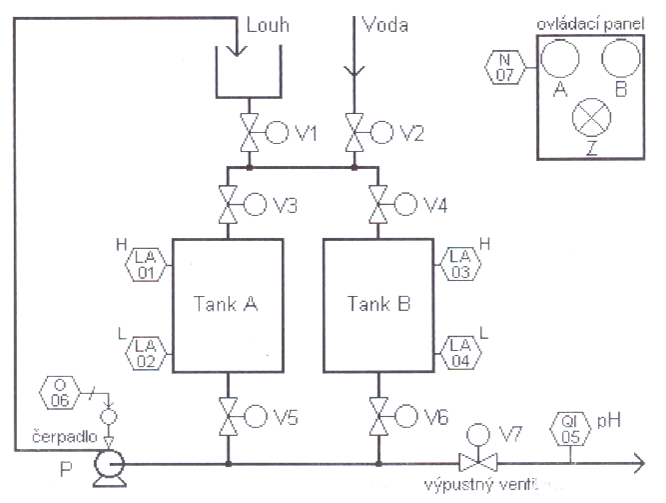
\includegraphics[width=0.6\textheight]{schema}
		\caption{Technologické schéma}
		\label{fig:schema}
	\end{figure}
	
	% Analýza úlohy
	\chapter{Analýza úlohy}
	
	\section{Stavy modelu}
	\begin{table}[]
		\begin{tabular}{ll}
			\hline
			\multicolumn{1}{c}{Stav} 	 & \multicolumn{1}{c}{Popis}      \\ \hline
			0                            & Počáteční stav				  \\
			1                            & Nádrže nejsou prázdné          \\
			2                            & Ruční vypouštění nádrže A   	  \\ 
			3                            & Ruční vypouštění nádrže B   	  \\ 
			4                            & Systém čeká na vstup 		  \\ \hline
			5A                           & Napouštění louhem nádrže A     \\
			6A                           & Vypouštění louhu nádrže A      \\
			7A                           & Napouštění vodou nádrže A      \\
			8A                           & Proplachování vodou nádrže A   \\
			9A                           & Vypouštění vody nádrže A       \\ \hline
			5B                           & Napouštění louhem nádrže B     \\
			6B                           & Vypouštění louhu nádrže B      \\
			7B                           & Napouštění vodou nádrže B      \\
			8B                           & Proplachování vodou nádrže B   \\
			9B                           & Vypouštění vody nádrže B       \\ \hline
		\end{tabular}
	\end{table}
	
	\section{Vstupní signály}
	\begin{table}[]
		\begin{tabular}{lll}
			\hline
			\multicolumn{1}{c}{Vstupní signál} 	& \multicolumn{1}{c}{Druh} & \multicolumn{1}{c}{Popis}  \\ \hline
			N\_A                                & Aktivní                  & Spuštění sanitace nádrže A \\
			N\_B                                & Aktivní                  & Spuštění sanitace nádrže B \\
			LA1\_i                              & Pasivní                  & Horní mez hladiny nádrže A \\
			LA2\_i                              & Pasivní                  & Dolní mez hladiny nádrže A \\
			LA3\_i                              & Pasivní                  & Horní mez hladiny nádrže B \\
			LA4\_i                              & Pasivní                  & Dolní mez hladiny nádrže B \\
			Q\_i                                & Pasivní                  & Kontrola pH na výtoku      \\
			RUC                                 & Aktivní                  & Ruční vypouštění nádrží    \\ \hline
		\end{tabular}
	\end{table}
	
	\section{Řídící signály}
	\begin{table}[]
		\begin{tabular}{ll}
			\hline
			\multicolumn{1}{c}{Řídící signál} 	& \multicolumn{1}{c}{Popis}  	\\ \hline
			V1\_i          					  	& Ventil 1      			   	\\
			V2\_i         					  	& Ventil 2      				\\
			V3\_i          					  	& Ventil 3      				\\
			V4\_i          					  	& Ventil 4      				\\
			V5\_i          					  	& Ventil 5      				\\
			V6\_i          					  	& Ventil 6      				\\
			V7\_i          					  	& Ventil 7      				\\
			P\_i          					  	& Čerpadlo      				\\
			Z\_i          					  	& Žárovka      					\\ \hline
		\end{tabular}
	\end{table}
	
	% Automatový model
	\chapter{Automatový model}
	
	% Implementace
	\chapter{Implementace}
	
	% Uživatelská příručka
	\chapter{Uživatelská příručka}
	
	% Závěr
	\chapter{Závěr}
	
\end{document}
